\documentclass[oneside,a4paper]{report}
\usepackage{color}
\usepackage{longtable}
\usepackage{titlesec}
\usepackage[hidelinks]{hyperref}
\usepackage{ulem}
\usepackage{float}
\usepackage{graphicx}
\usepackage{fancyhdr}
\usepackage{rotating}
\usepackage[T1]{fontenc}
\usepackage[headheight=25pt,margin=0.7in,top=1.5in,bottom=1in,right=1in,left=1in]{geometry}

\hypersetup{colorlinks=true,linktoc=none,citecolor=black,urlcolor=blue}
\hypersetup{linktocpage=false,linkcolor=black}

\pagestyle{fancy}
\fancyhead[R]{
\includegraphics[width=2cm]{./latex/resources/kitlogo.png}}
\fancyhead[L]{\leftmark}

\fancypagestyle{plain}{
        \rhead{
\includegraphics[width=2cm]{./latex/resources/kitlogo.png}}
        \lhead{\leftmark}
}


\renewcommand{\arraystretch}{2}

\titleformat{\chapter}[hang]
 {\normalfont\bfseries\LARGE}{\thechapter. }{0pt}{\LARGE}
\titleformat{\section}[hang]
 {\normalfont\bfseries\Large}{\thesection. }{0pt}{\Large}
\titleformat{\paragraph}[hang]
 {\normalfont\bfseries\normalsize}{}{}{}

\titlespacing*{\chapter}{0pt}{-20pt}{10pt}

\begin{document}
	\begin{titlepage}
	\centering
	{\scshape\LARGE Karlsruhe Institute of Technology \par}
	\vspace{1cm}
	{\scshape\Large Software Engineering Practice\par}
	\vspace{0.5cm}
	{\scshape\Large WINTER TERM 2015/2016\par}
	\vspace{1.5cm}
	{\Huge\bfseries rootJS - Implementation Report\par}
	\vspace{0.25cm}
	{\Large\bfseries Node.js bindings for ROOT 6\par}
	\vspace{2cm}
	{\Large\itshape Jonas Schwabe\par}
	{\Large\itshape Theo Beffart\par}
	{\Large\itshape Sachin Rajgopal\par}
	{\Large\itshape Christoph Wolff\par}
	{\Large\itshape Christoph Haas\par}

	{\Large\itshape Maximilian Fr\"uh\par}
	\vfill
	supervised by\par
	Dr.~Marek \textsc{Szuba}

	\vfill

	% Bottom of the page
	{\large \date{99.99.9999}\par}
\end{titlepage}

  	\tableofcontents
	\chapter{Introduction}
\section{About rootJS}
The purpose of creating Node.js bindings of ROOT, called rootJS, is to enable users to 
integrate ROOT in Node.js programs, such as Node.js based web servers. 
	\chapter{Architecture}
\section{The class diagrams in comparison}
	\begin{figure}[H]
	\centering
	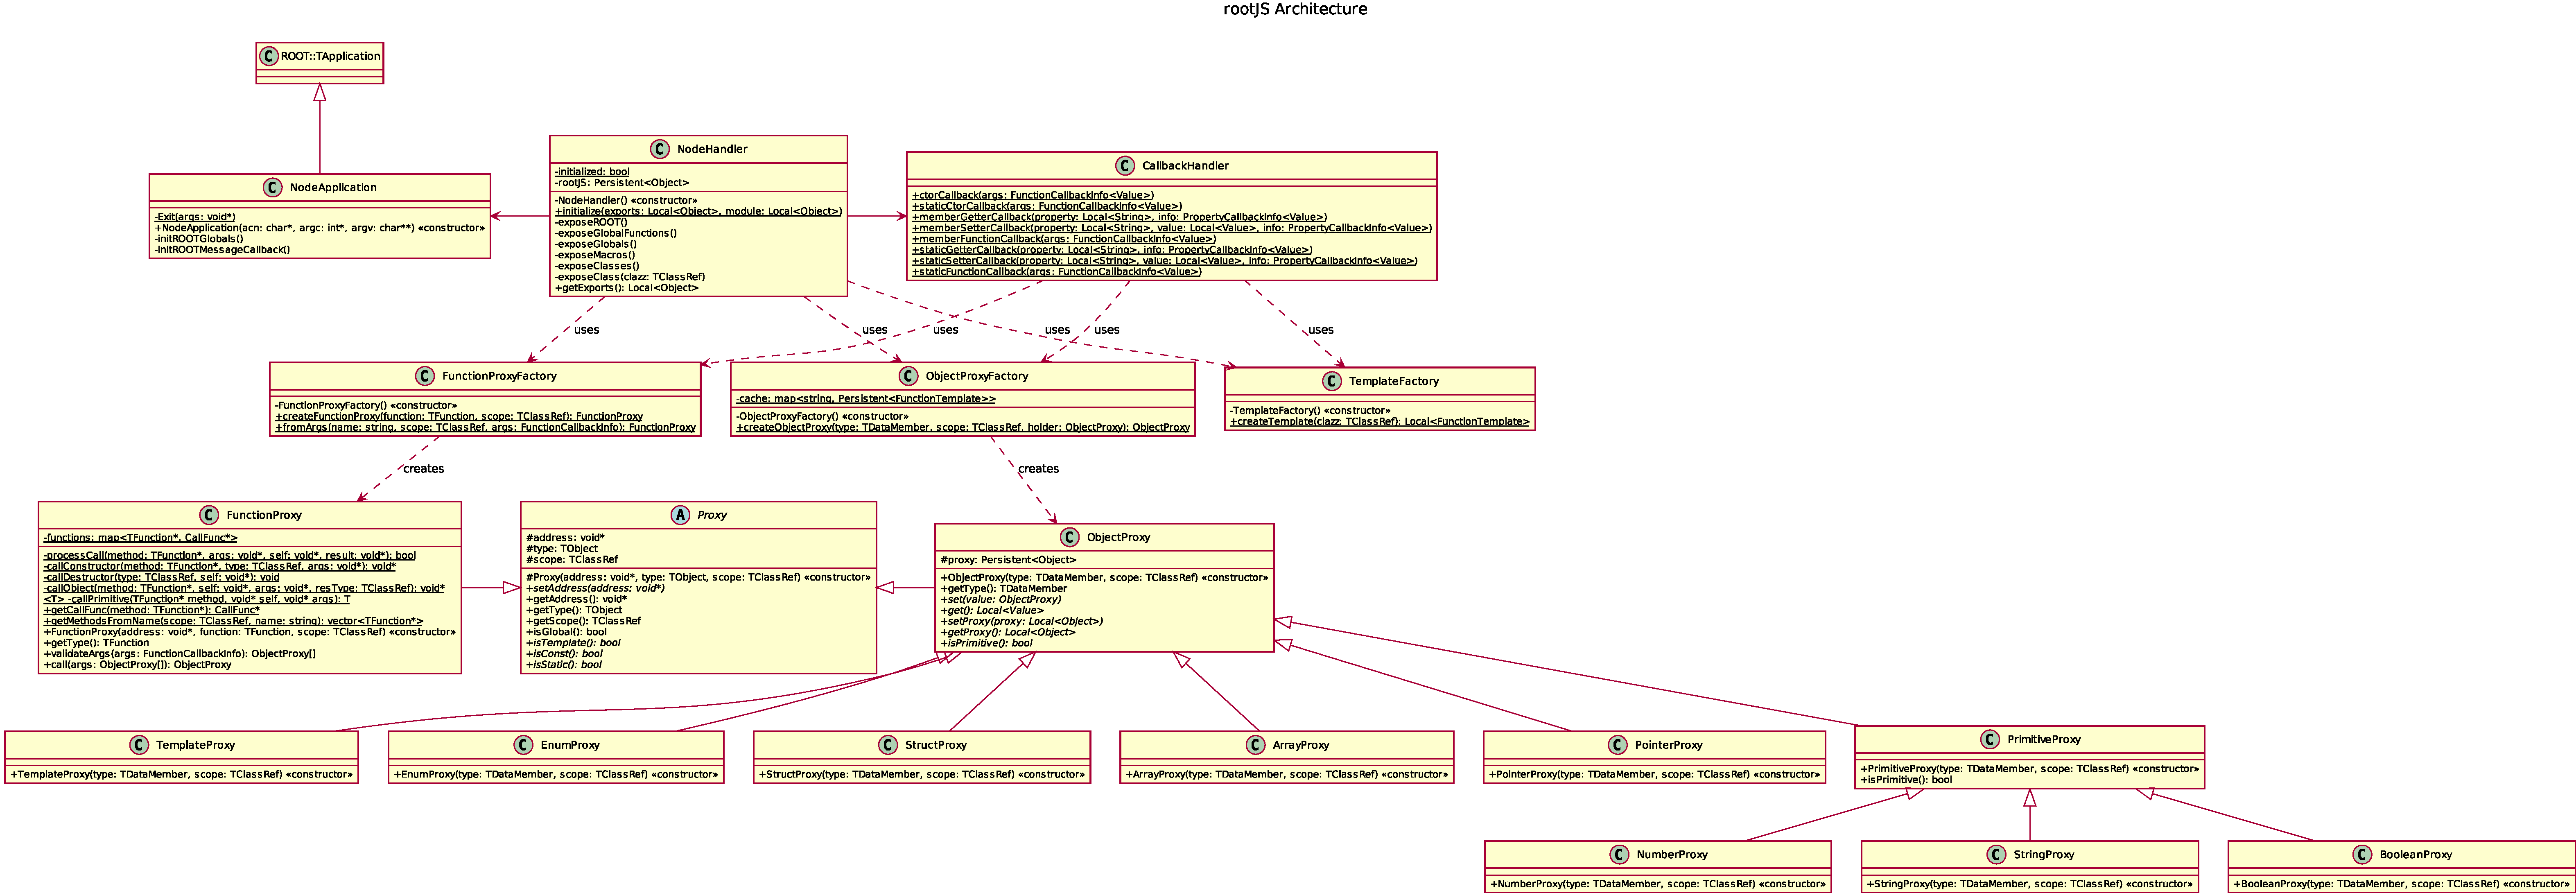
\includegraphics[keepaspectratio=true, width=7.75in, 
	angle=90]{./latex/oldResources/architecture.pdf}
	\caption{The rootJS class diagram at the conclusion of the design phase}
\end{figure}


\begin{figure}[H]
	\centering
	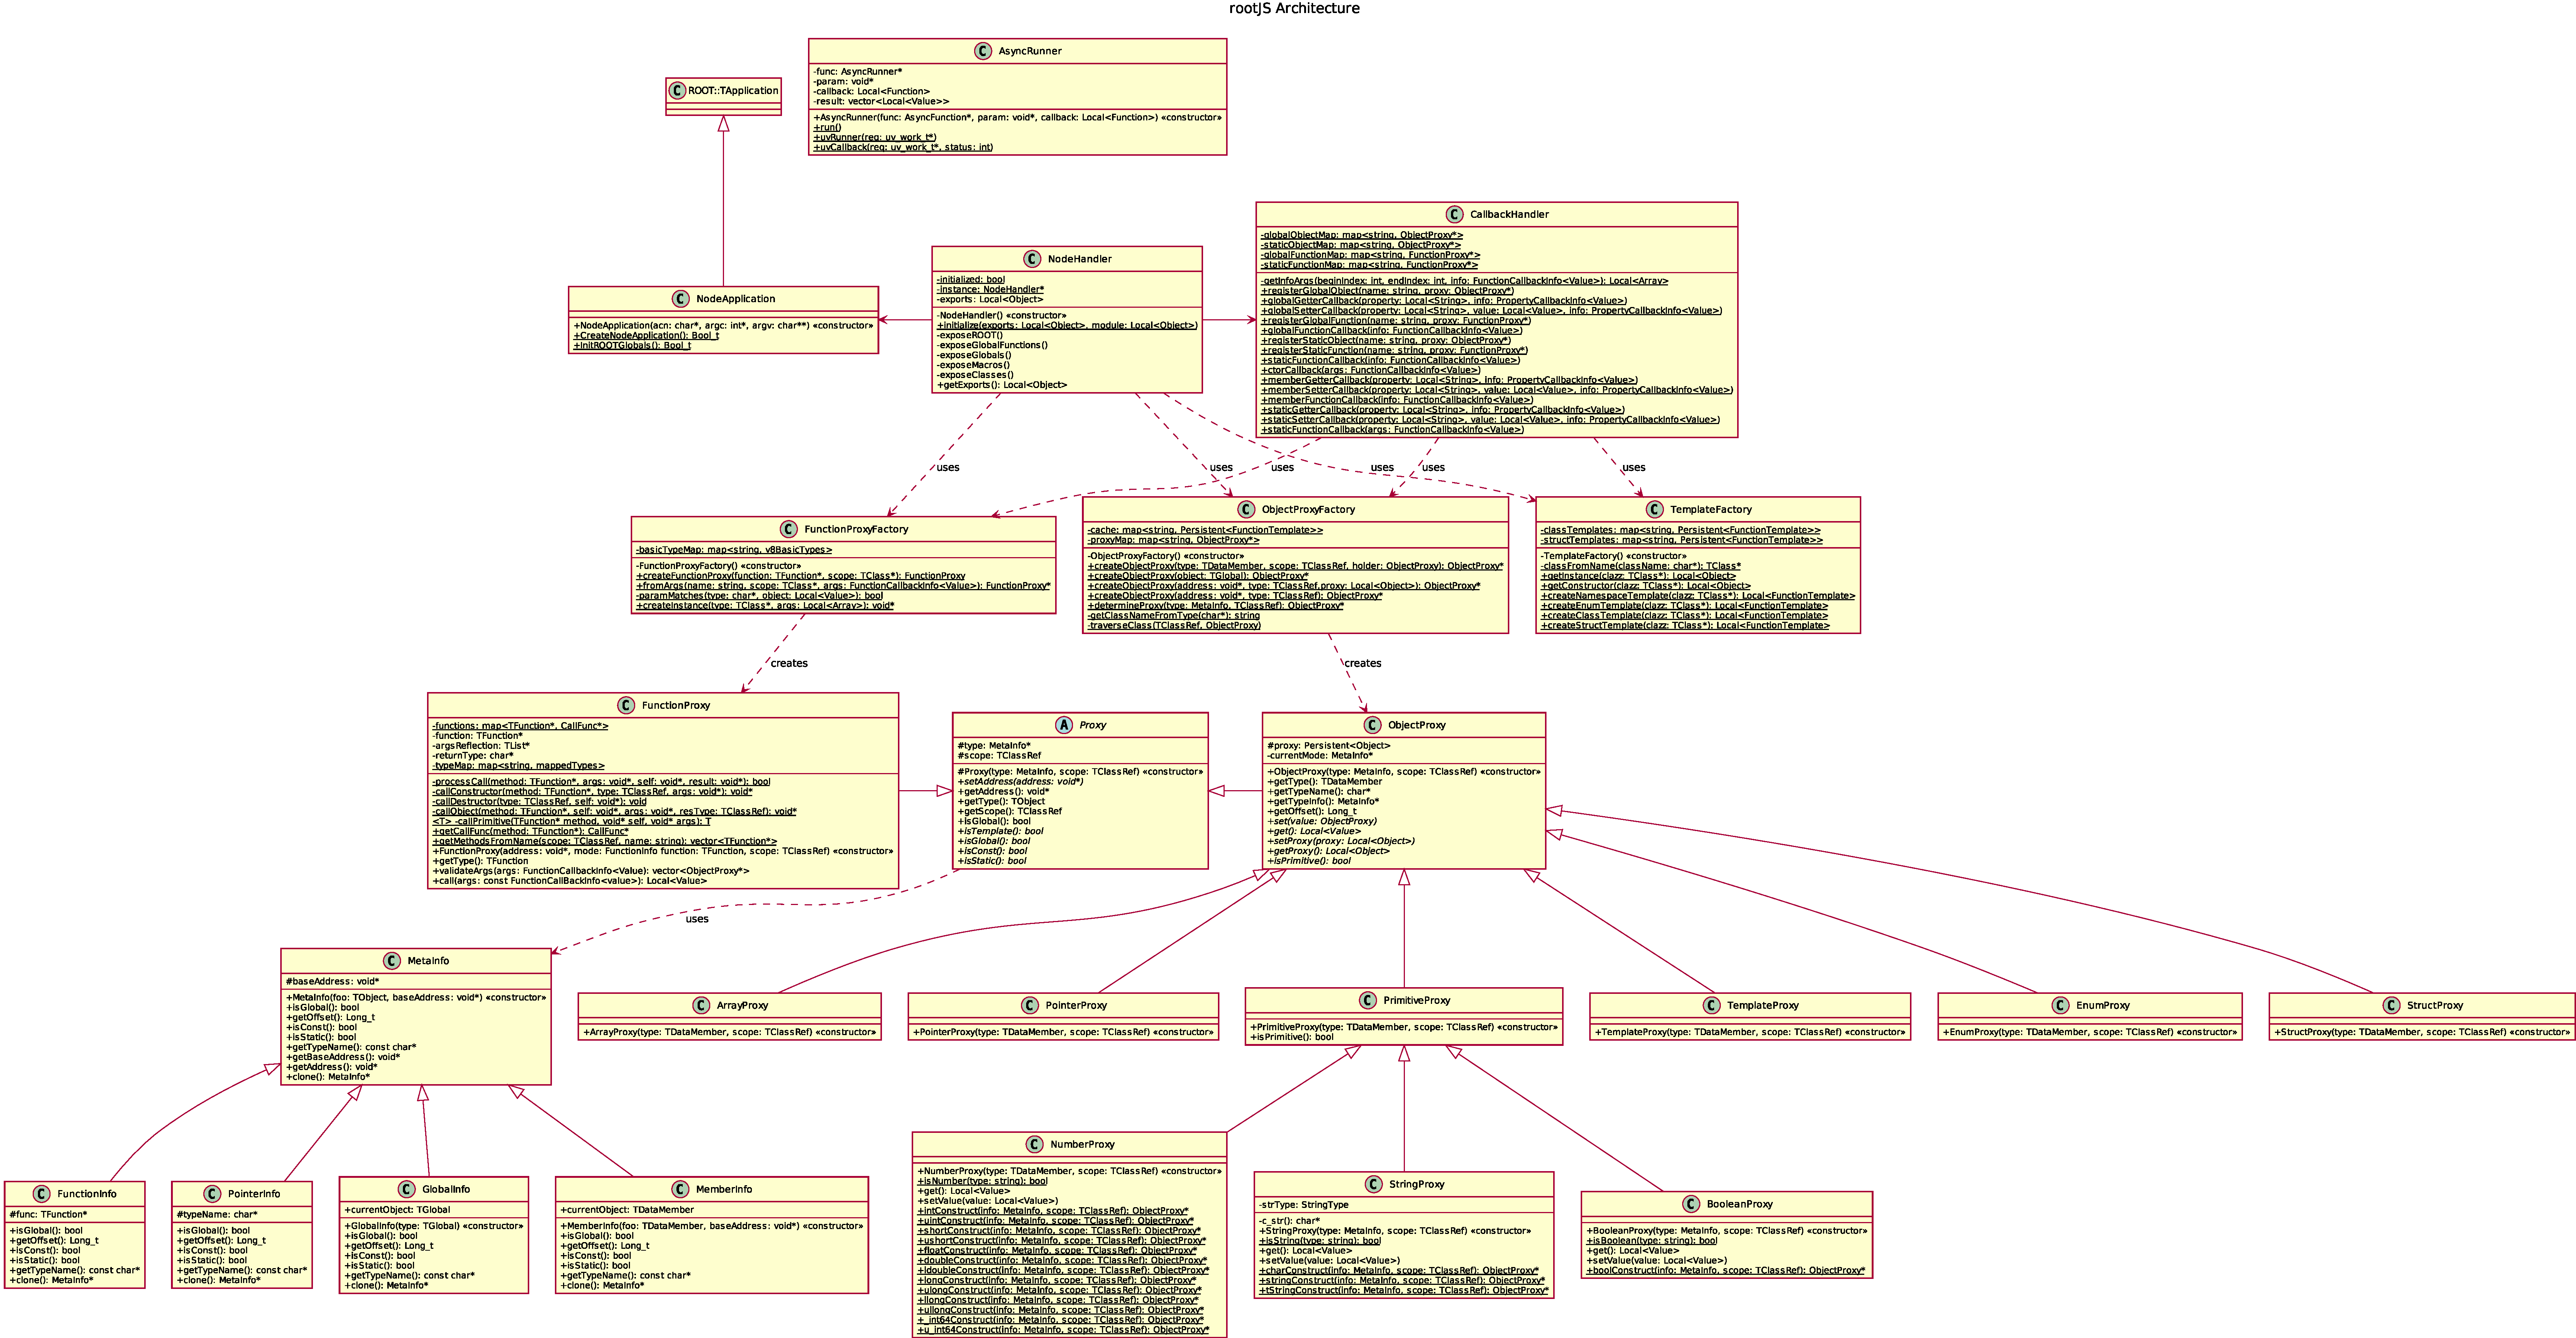
\includegraphics[keepaspectratio=true, width=9in,
	 angle=90]{./latex/resources/architecture.pdf}
	\caption{The current rootJS class diagram }
\end{figure}
\section{The Changes in the Architecture in detail}
\begin{itemize}
	\item MetaInfo
\end{itemize}
The MetaInfo class and its subclasses MemberInfo, GlobalInfo, PointerInfo and FunctionInfo were added to encapsulate the 
differences between TGlobals and TDataMembers. In the initial design, an ObjectProxy would have had to handle
both TGlobals and TDataMembers, but there subtle differences between them. One of them would be that TDataMembers 
have an offset while TGlobals do not. Therefore there was a need to create a class which contains the specific information 
of them. Later it turned out that TFunctions and pointers also require an information class. 
Now an ObjectProxy instance can only be created with the constructor if a MetaInfo class is passed as a parameter.
\begin{itemize}
	\item AsyncRunner
\end{itemize}

\begin{itemize}
	\item TemplateFactory
\end{itemize}
\begin{itemize}
	\item FunctionProxyFactory
\end{itemize}
\begin{itemize}
	\item clone() and backup()
\end{itemize}
\begin{itemize}
	\item ObjectProxyFactory
\end{itemize}
\begin{itemize}
	\item primitives construct methods
\end{itemize}




	\chapter{Criteria}
\section{Required Criteria}
These are the Required Criteria as stated in the functional specification:
\begin{itemize}
	\item work on Linux
\end{itemize}
	This is rather straightforward as long as the user has installed the required dependencies. 
	This means that, at the very least, ROOT and Node.js have to be installed. 
	ROOT is supported on only a few major Linux distributions, so rootJS is limited to the systems
	on which ROOT has been installed.
	
\begin{itemize}
	\item allow the user to interact with any ROOT class from the Node.js JavaScript interpreter
\end{itemize}
	The user is able to interact with any ROOT class by requesting any class with rootJS. The following is an extract from the description of the NodeHandler	in the module guide, which describes how rootJS is started up:
\begin{verbatim}
// JavaScript: Load ROOT bindings in JavaScript
var root = require(rootJS.node);

// C++: Expose the initialize method as the main entry point
NODE_MODULE(rootJS, initialize)
\end{verbatim}
	A file \textit{index.js} is offered to make initializing rootJS easier for the user 
	which will also handle user interface callbacks. \\
	\\
	\textit{index.js} :
\begin{verbatim}	
module.exports = require('./build/Release/rootjs.node');

var uicallback = function() {
	module.exports.gSystem.ProcessEvents();
	setTimeout(uicallback, 100);
}
uicallback();
\end{verbatim}
	If the user would then like to open a TBrowser() from ROOT, then they would have to do the following: 
\begin{verbatim}
var root = require('./index.js');
new root.TBrowser();
\end{verbatim}
	The user would then have access to a  TBrowser() from ROOT. 
	
\begin{itemize}
	\item accept C++ code for just-in-time compilation
\end{itemize}
The user will have access to the Node.js interpreter and can enter single lines of code in it. 
These lines of code will be interpreted by rootJS and rootJS will call Cling to interpret them.

\begin{itemize}
	\item update dynamically following changes to C++ internals
\end{itemize}


\begin{itemize}
	\item provide asynchronous wrappers for common I/O operations (i.e. file and tree access)
\end{itemize}
While no specifics were written about asynchronous processes in the module guide, two variations were considered. The first variation would utilize ROOT's inbuilt 
multi-threading environment. ROOT contains a TThread class which is similar to the std::thread class in C++, but is adjusted to ROOT. 
The second variation would use libuv, a software library that provides asynchronous even notification and was mainly designed for Node.js. 

\section{Optional Criteria}
These are the Optional Criteria as stated in the functional specification:
\begin{itemize}
	\item support the streaming of data in JavaScript Object Notation (JSON) format compatible with JavaScript ROOT
\end{itemize}


\begin{itemize}
	\item implement a web server based on Node.js to mimic the function of the ROOT HTTP server
\end{itemize}


\begin{itemize}
	\item work OS independent (i.e. support Mac OS X, Linux operating systems)
\end{itemize}

\section{Limiting Criteria}
These are the Limiting Criteria as stated in the functional specification:
\begin{itemize}
	\item add any extending functionality to the existing ROOT framework
\end{itemize}
No code was written to implement any new features which are not already existing in the ROOT framework. 

\begin{itemize}
	\item necessarily support previous ROOT versions
\end{itemize}
ROOT 6 uses the LLVM-based C++ interpreter Cling, while ROOT 5.34 uses the C++ interpreter CINT. 
rootJS was designed with ROOT 6 in mind and many of the function calls, etc. will only work with Cling. 
As of yet, rootJS has not been tested not been test on older ROOT versions, but it is very unlikely that rootJS will function with ROOT 5.34.

\begin{itemize}
	\item necessarily support future ROOT versions
\end{itemize}
If future versions of ROOT also utilize Cling, rootJS might be able to support them. Therefore it is likely that rootJS should support all versions of ROOT 6.

	\chapter{Unit Tests}
%  \clearpage


\end{document}
